\let\negmedspace\undefined
\let\negthickspace\undefined
\documentclass[journal]{IEEEtran}
\usepackage[a5paper, margin=10mm, onecolumn]{geometry}
\usepackage{lmodern} % Ensure lmodern is loaded for pdflatex
\usepackage{tfrupee} % Include tfrupee package

\setlength{\headheight}{1cm} % Set the height of the header box
\setlength{\headsep}{0mm}     % Set the distance between the header box and the top of the text


\usepackage{gvv}
\usepackage{cite}
\usepackage{amsmath,amssymb,amsfonts,amsthm}
\usepackage{algorithmic}
\usepackage{graphicx}
\usepackage{textcomp}
\usepackage{xcolor}
\usepackage{txfonts}
\usepackage{listings}
\usepackage{enumitem}

\usepackage{gensymb}
\usepackage{comment}
\usepackage[breaklinks=true]{hyperref}
\usepackage{tkz-euclide} 
\usepackage{listings}
% \usepackage{gvv}
\def\inputGnumericTable{}
\usepackage[latin1]{inputenc}
\usepackage{color}
\usepackage{array}
\usepackage{longtable}
\usepackage{calc}
\usepackage{multirow}
\usepackage{hhline}
\usepackage{ifthen}
\usepackage{lscape}
\begin{document}

\bibliographystyle{IEEEtran}
\vspace{3cm}

\title{1-1.5-19}
\author{EE24BTECH11003 - Akshara Sarma Chennubhatla}
% \maketitle
% \newpage
% \bigskip
{\let\newpage\relax\maketitle}

\renewcommand{\thefigure}{\theenumi}
\renewcommand{\thetable}{\theenumi}
\setlength{\intextsep}{10pt} % Space between text and floats


\numberwithin{equation}{enumi}
\numberwithin{figure}{enumi}
\renewcommand{\thetable}{\theenumi}

\textbf{Question:} \\Find the ratio in which the segment joining the points \brak{1,3} and \brak{4, 5} is divided by the $X$ axis. Also find the coordinates of this point on the $X$ axis.
Using section formula,\\
\begin{table}[h!]    
  \centering
  \begin{tabular}[12pt]{ |c| c|}
    \hline
    \textbf{Variable} & \textbf{Description}\\ 
    \hline
    $\vec{P}$ & Point on the $X$-axis\\
    \hline
    $\vec{A}$ & $\myvec{1\\3}$ point\\
    \hline
    $\vec{B}$ & $\myvec{4\\5}$ point\\
    \hline
    $\vec{k}$ & ratio in which $P$ divides $AB$ to be found\\
    \hline
\end{tabular}

  \caption{Variables Used}
  \label{tab1-1.5-19}
\end{table}
\solution
\begin{align}
\myvec{x\\0}&=\frac{\myvec{1\\3}+k\myvec{4\\5}}{1+k}\\
\implies \frac{5k+3}{k+1}&=0\\
\implies k&=\frac{-3}{5}\\
x&=\frac{1}{k+1}+\frac{4k}{k+1}\\
\implies x&=\frac{1+4\brak{\frac{-3}{5}}}{\brak{\frac{-3}{5}}+1}\\
\implies x&=\frac{-7}{2}
\end{align}
Therefore the ratio in which the line segment joining the points \brak{1,3} and \brak{4,5} is divided by the $X$ axis is $-3:5$. The point on the $X$ axis which divides the line segment in the ratio is $\brak{\frac{-7}{2},0}$
\begin{figure}[h!]
\centering
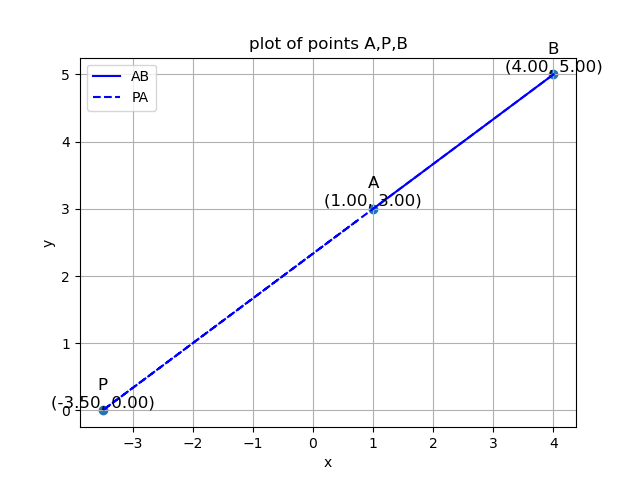
\includegraphics[width=0.7\columnwidth]{figs/figure.png}	
\label{Plot of points A,B and P and the line joining them}
\end{figure}
\end{document}
